% ============================================================
%  Section 3 — Methodology
%  Describes the proposed framework in generic terms (notation,
%  equations, design rationale). Dataset-specific values (window
%  length, thresholds, partition sizes) and hyperparameters are
%  given in Section 4; all measured outcomes are in Section 5.
%
%  Packages needed (preamble): amsmath, amssymb, algorithm,
%  algpseudocode, graphicx, booktabs.
%
%  Figure needed: figures/framework_overview.png (Lucid export)
% ============================================================

\section{Methodology}
\label{sec:methodology}

This section presents the proposed framework. Its overall structure
is given first, followed by the notation, the automatic construction
of degradation stages and RUL targets, and the three contributions:
stage-conditioned generative augmentation, multi-task prediction, and
stage-conditional conformal calibration.

% ------------------------------------------------------------
\subsection{Framework Overview}
\label{sec:method_overview}

Fig.~\ref{fig:framework} summarises the framework. Raw vibration
recordings are first converted into multivariate feature vectors and
a scalar health indicator. The health indicator is used to place two
landmarks on each bearing's trajectory, the First Prediction Time and
an acceleration point, which define three degradation stages and a
piecewise RUL target without manual annotation. The feature vectors
are then segmented into fixed-length windows, and the bearings are
divided into training, validation, calibration and test partitions.\\

The three contributions act at successive points of this pipeline.
The stage-conditioned generator (C1) is trained on the training
partition and produces synthetic near-failure windows, which enter
the training set only. The multi-task predictor (C2) is trained on
this augmented set to estimate the RUL and the degradation stage
jointly from a shared representation. Finally, the stage-conditional
conformal procedure (C3) uses the real calibration partition to turn
each point prediction into an interval with a coverage guarantee
within each degradation stage.\\

One constraint governs the whole pipeline: synthetic data never
reaches the calibration or test partitions. The coverage guarantee of
conformal prediction rests on the calibration and test samples being
exchangeable. Synthetic windows follow the distribution learned by the
generator, not the true data distribution, so admitting them into
calibration would measure the predictor's error against the wrong
reference. Augmentation is therefore confined to training, where it
can only change the predictor, and the guarantee is preserved.

\begin{figure*}[!htbp]
  \centering
  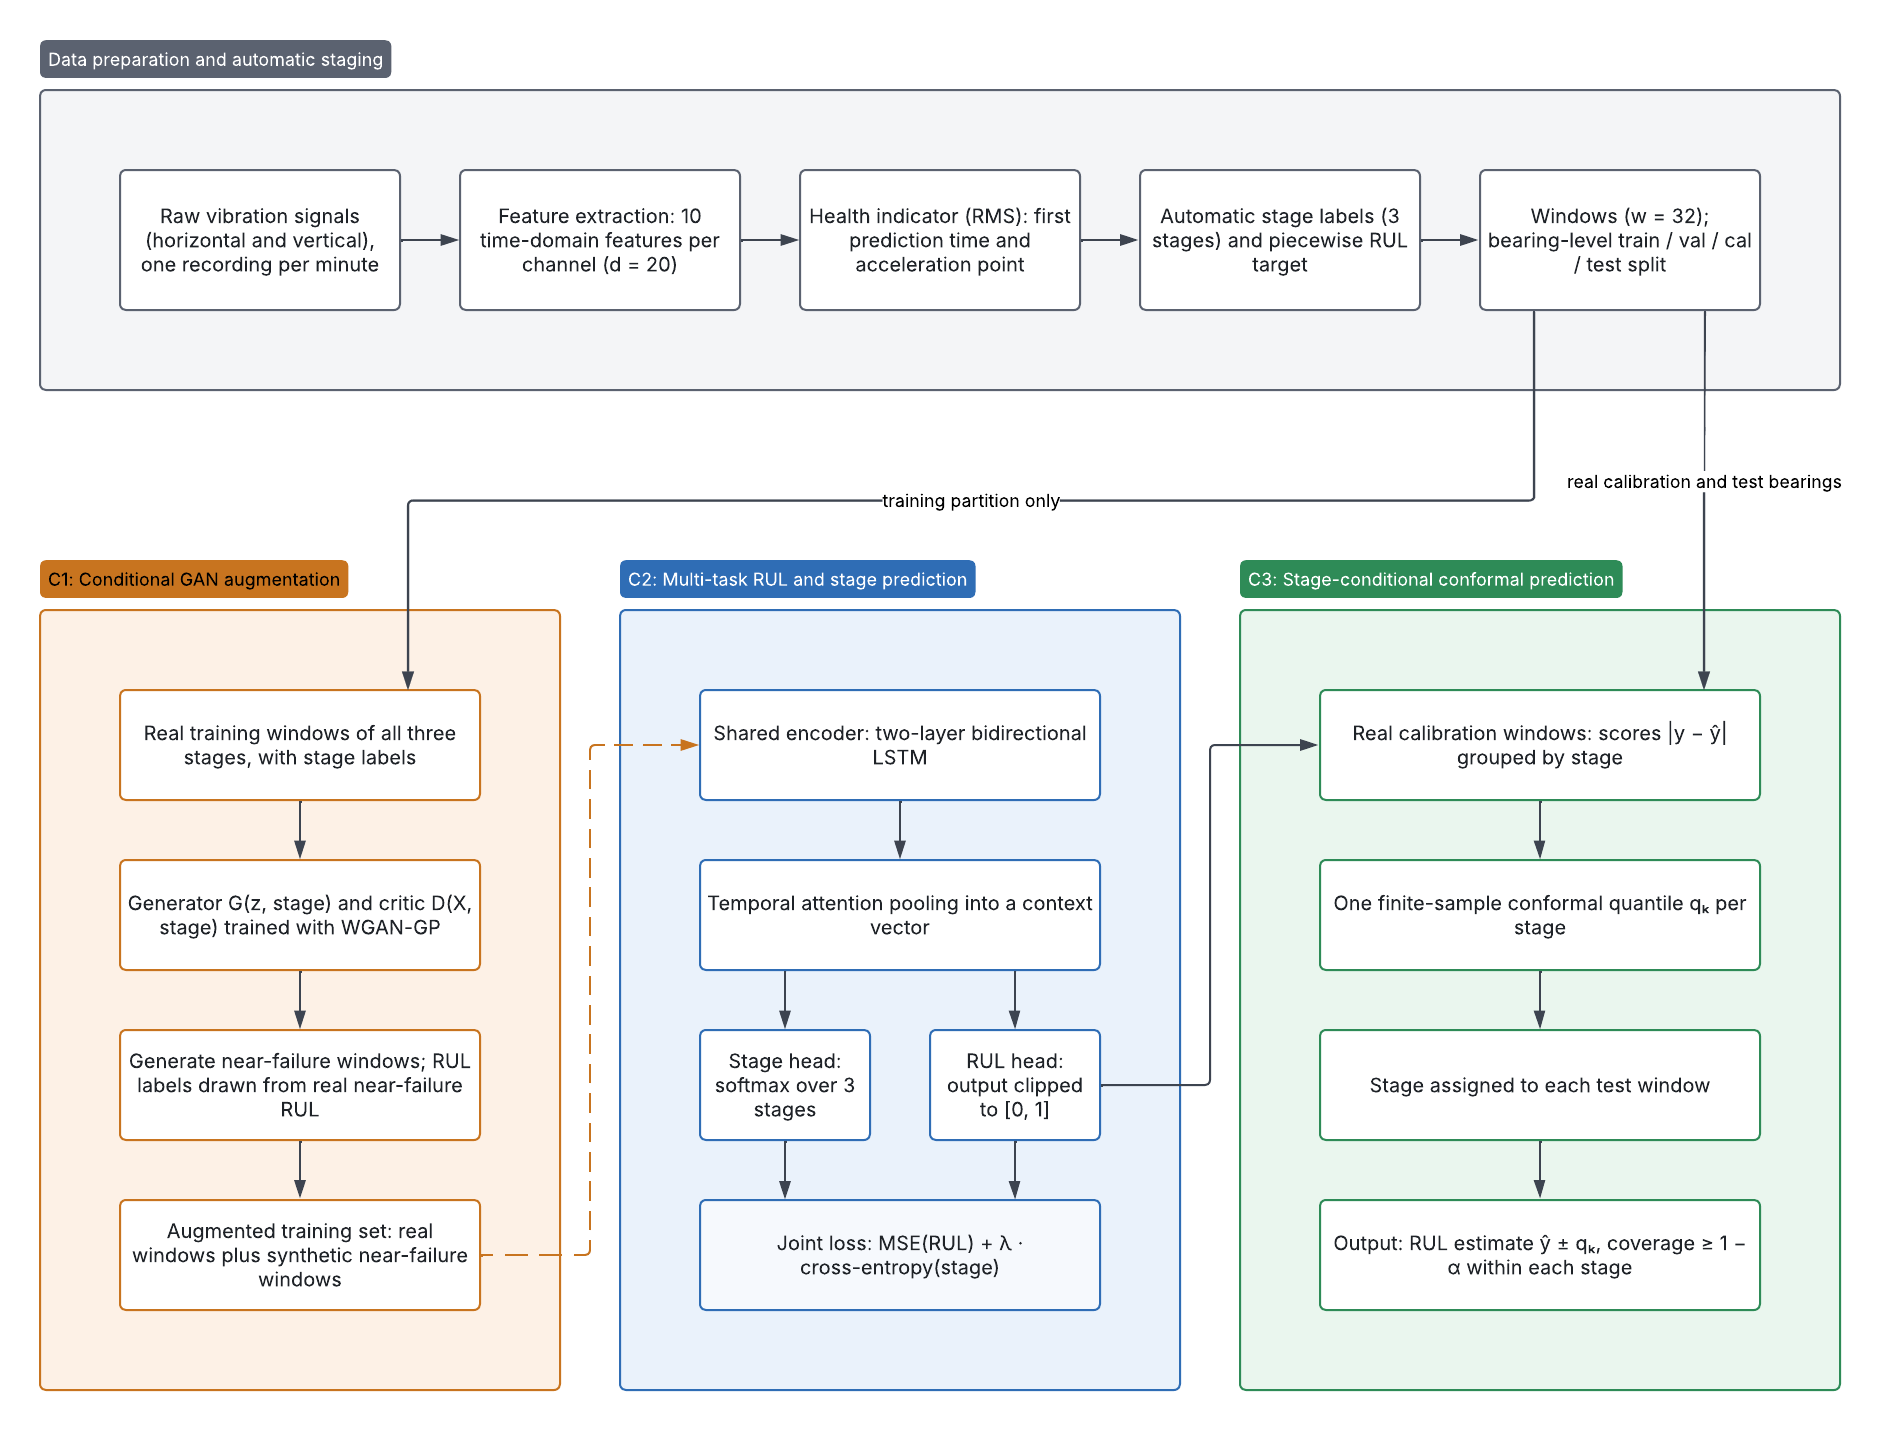
\includegraphics[width=\textwidth]{figures/framework_overview.png}
  \caption{Overview of the proposed framework. Synthetic windows
  produced by the stage-conditioned generator (C1) enter the training
  set only (dashed arrow); the calibration and test partitions contain
  real recordings exclusively. The trained RUL head of the multi-task
  predictor (C2) supplies the point estimates whose calibration
  residuals define the stage-wise conformal quantiles (C3).}
  \label{fig:framework}
\end{figure*}

% ------------------------------------------------------------
\subsection{Problem Formulation}
\label{sec:method_notation}

Consider a set of bearings $\mathcal{B}$, each monitored from its
first recording to failure. For bearing $b \in \mathcal{B}$ with
lifetime $T_b$ recordings, a feature vector
$\mathbf{x}^{b}_{t} \in \mathbb{R}^{d}$ is extracted from the
recording at time $t = 1, \dots, T_b$. The model input at time $t$ is
the window of the $w$ most recent feature vectors,
\begin{equation}
  \mathbf{X}^{b}_{t} =
  \left[\mathbf{x}^{b}_{t-w+1}, \dots, \mathbf{x}^{b}_{t}\right]
  \in \mathbb{R}^{w \times d}, \qquad t \geq w,
  \label{eq:window}
\end{equation}
which contains no information posterior to $t$. Each window carries
two labels taken at its final time step: a normalised RUL target
$y^{b}_{t} \in [0,1]$ and a degradation stage
$s^{b}_{t} \in \{1, 2, 3\}$, both defined in
Section~\ref{sec:method_staging}.\\

The bearings are split into disjoint training, validation,
calibration and test sets, denoted $\mathcal{D}_{\mathrm{tr}}$,
$\mathcal{D}_{\mathrm{val}}$, $\mathcal{D}_{\mathrm{cal}}$ and
$\mathcal{D}_{\mathrm{te}}$, at the level of whole bearings. This
choice follows from Eq.~\eqref{eq:window}: consecutive windows of the
same bearing share $w-1$ of their $w$ time steps, so a window-level
split would place near-duplicates on both sides of the
training--calibration boundary.\\

The objective is twofold. The first is a point predictor
$\hat{f}: \mathbb{R}^{w \times d} \to [0,1]$ with small error on
unseen bearings, particularly in the near-failure stage. The second is
an interval predictor $\hat{C}(\mathbf{X})$ that satisfies, for a
user-chosen miscoverage level $\alpha$, the stage-conditional coverage
property
\begin{equation}
  \mathbb{P}\left( y \in \hat{C}(\mathbf{X}) \;\middle|\; s = k \right)
  \geq 1 - \alpha, \qquad k \in \{1, 2, 3\}.
  \label{eq:coverage_goal}
\end{equation}
Coverage within each stage is required, rather than coverage averaged
over all windows, because the stages differ sharply in size and
difficulty. An average dominated by the abundant healthy windows can
satisfy the nominal level while the near-failure stage, the one that
drives maintenance decisions, is under-covered.

% ------------------------------------------------------------
\subsection{Automatic Degradation Staging and RUL Target}
\label{sec:method_staging}

Stage labels and RUL targets are derived from a scalar health
indicator (HI) rather than annotated by hand. The HI $h_t$ is the root
mean square of one vibration channel, computed per recording and
smoothed with a short moving average.\\

The First Prediction Time $t_{\mathrm{F}}$ marks the end of the healthy
regime. A healthy baseline with mean $\mu_b$ and standard deviation
$\sigma_b$ is estimated from the initial fraction $\eta$ of the
bearing's life. The detection threshold is the stricter of a
statistical criterion and a relative floor,
\begin{equation}
  \tau_b = \max\left( \mu_b + 3\sigma_b,\; (1+\rho)\,\mu_b \right),
  \label{eq:fpt_threshold}
\end{equation}
and the FPT is the first instant from which the HI stays above
$\tau_b$ for $m$ consecutive recordings,
\begin{equation}
  t_{\mathrm{F}} = \min \left\{ t \;:\; h_{t+j} > \tau_b,
  \;\; j = 0, \dots, m-1 \right\}.
  \label{eq:fpt}
\end{equation}
The two terms of Eq.~\eqref{eq:fpt_threshold} play distinct roles. The
statistical term rejects departures that are small compared with the
baseline noise. The relative term $\rho$ guards against bearings whose
baseline is so stable that $\sigma_b$ is close to zero, in which case
$\mu_b + 3\sigma_b$ alone would be crossed by ordinary fluctuations.
The persistence length $m$ in Eq.~\eqref{eq:fpt} prevents a single
transient from being taken as a change of regime.\\

Within the degradation phase, an acceleration point $t_{\mathrm{A}}$
separates gradual from severe degradation. Let
$\Delta h_t = h_t - h_{t-1}$ denote the first difference of the HI.
Its mean $\mu_\Delta$ and standard deviation $\sigma_\Delta$ are
estimated over the first half of the interval
$[t_{\mathrm{F}}, T_b]$, and $t_{\mathrm{A}}$ is the first instant in
the second half at which
\begin{equation}
  \Delta h_t > \mu_\Delta + \sigma_\Delta .
  \label{eq:acc_point}
\end{equation}
When no such instant exists, $t_{\mathrm{A}}$ is placed at 70\% of the
degradation interval. The two landmarks define the stage of every
recording,
\begin{equation}
  s_t =
  \begin{cases}
    1 & t < t_{\mathrm{F}} \quad \text{(healthy)},\\
    2 & t_{\mathrm{F}} \leq t < t_{\mathrm{A}}
        \quad \text{(early degradation)},\\
    3 & t \geq t_{\mathrm{A}} \quad \text{(near-failure)}.
  \end{cases}
  \label{eq:stages}
\end{equation}

The RUL target is defined piecewise from the same landmark:
\begin{equation}
  y_t =
  \begin{cases}
    1 & t < t_{\mathrm{F}},\\[2pt]
    \dfrac{T_b - t}{T_b - t_{\mathrm{F}}} & t \geq t_{\mathrm{F}}.
  \end{cases}
  \label{eq:rul_target}
\end{equation}
The target is held at unity during the healthy phase and decreases
linearly to zero at failure. A target that decreases from the first
recording would give different labels to healthy windows whose
signals are nearly identical, a mapping the predictor cannot learn.
Because healthy windows are the most numerous, such a target also
biases the predictor toward overestimating the remaining life, which
is the unsafe direction of error. Normalising by the length of the
degradation phase keeps the target on a common scale across bearings
whose lifetimes may differ by orders of magnitude.

% ------------------------------------------------------------
\subsection{Stage-Conditioned Generative Augmentation (C1)}
\label{sec:c1_gan}

The near-failure stage is the least represented in run-to-failure data
and the most important for maintenance. C1 enlarges it with synthetic
windows produced by a conditional generative adversarial network. The
generator produces complete multivariate windows of dimension
$w \times d$, rather than a scalar degradation curve, so that the
correlations between features and between channels are reproduced.\\

\textit{Architecture.} The generator $G$ receives a noise vector
$\mathbf{z} \sim \mathcal{N}(\mathbf{0}, \mathbf{I})$ concatenated with
a one-hot encoding $\mathbf{e}_c$ of the requested stage $c$. A linear
layer projects this input into a short seed sequence, two
one-dimensional convolutional layers extract local patterns, and a
bidirectional LSTM models the temporal dependencies before a linear
layer outputs the window $\tilde{\mathbf{X}} = G(\mathbf{z},
\mathbf{e}_c)$. The critic $D$ receives a window together with the same
stage encoding, repeated at every time step, and passes it through two
convolutional layers and a bidirectional LSTM. The final hidden state
is layer-normalised and mapped to an unbounded scalar score. Layer
normalisation is used instead of batch normalisation because the
gradient penalty below is defined per sample.\\

Conditioning both networks on the stage is what allows a specific
regime to be requested. An unconditional generator would reproduce the
distribution of its training data, which is dominated by healthy
windows, and leave the scarcity unaddressed. The generator is
therefore trained on windows of all three stages, so that it learns
how the stages differ, and is queried only for $c = 3$ at
augmentation time.\\

\textit{Training objective.} Training follows the Wasserstein
formulation with gradient penalty~\cite{NIPS2017_892c3b1c}, chosen for
its resistance to mode collapse. A collapsed generator would emit
near-identical windows and add no information to the training set.
The critic minimises
\begin{equation}
  \mathcal{L}_{D} =
  \mathbb{E}\big[ D(\tilde{\mathbf{X}}, \mathbf{e}_c) \big]
  - \mathbb{E}\big[ D(\mathbf{X}, \mathbf{e}_c) \big]
  + \lambda_{\mathrm{gp}}\,
  \mathbb{E}\Big[ \big( \lVert \nabla_{\hat{\mathbf{X}}}
  D(\hat{\mathbf{X}}, \mathbf{e}_c) \rVert_2 - 1 \big)^2 \Big],
  \label{eq:critic_loss}
\end{equation}
where $\mathbf{X}$ is a real window of stage $c$, $\tilde{\mathbf{X}}$
a generated window of the same stage, and
$\hat{\mathbf{X}} = \epsilon \mathbf{X} + (1-\epsilon)
\tilde{\mathbf{X}}$ with $\epsilon \sim \mathcal{U}(0,1)$. The last
term enforces the Lipschitz constraint on which the Wasserstein
estimate depends. The generator minimises
\begin{equation}
  \mathcal{L}_{G} =
  - \mathbb{E}\big[ D(G(\mathbf{z}, \mathbf{e}_c), \mathbf{e}_c) \big],
  \label{eq:gen_loss}
\end{equation}
and is updated once for every $n_{\mathrm{c}}$ critic updates. A
separate generator is trained for each cross-validation fold, on that
fold's training windows only.\\

\textit{Augmentation and labelling.} Let $N_3$ be the number of real
near-failure windows in $\mathcal{D}_{\mathrm{tr}}$. For an
augmentation ratio $r$, the generator produces
$\lfloor r N_3 \rceil$ windows with $c = 3$, and these are added to the
training set with stage label 3. Each synthetic window also needs an
RUL label, which the generator does not provide because it is
conditioned on the stage and not on the RUL. The label is drawn at
random, with replacement, from the empirical distribution of the RUL
values of the real near-failure training windows,
\begin{equation}
  \tilde{y} \sim \mathrm{Unif}\left\{ y_i \;:\; s_i = 3,\;
  i \in \mathcal{D}_{\mathrm{tr}} \right\}.
  \label{eq:syn_label}
\end{equation}
This preserves the marginal distribution of near-failure RUL values in
the augmented set, so the augmentation does not shift the predictor
toward any particular value. The augmented set
$\mathcal{D}_{\mathrm{tr}}^{+} = \mathcal{D}_{\mathrm{tr}} \cup
\mathcal{D}_{\mathrm{syn}}$ replaces $\mathcal{D}_{\mathrm{tr}}$ for
training the predictor. The validation, calibration and test sets are
left unchanged.

% ------------------------------------------------------------
\subsection{Multi-task RUL and Stage Prediction (C2)}
\label{sec:c2_multitask}

The predictor estimates the RUL and the degradation stage jointly from
a shared encoder. The auxiliary stage task asks the encoder to
separate the three regimes, which are the same regimes in which the
RUL behaves differently. The stage labels come from
Eq.~\eqref{eq:stages} and therefore cost no annotation.\\

\textit{Shared encoder.} A two-layer bidirectional LSTM maps the input
window to a sequence of hidden states
$\mathbf{H} = [\mathbf{h}_1, \dots, \mathbf{h}_w]$, where each
$\mathbf{h}_k$ concatenates the forward and backward states. A temporal
attention layer pools this sequence into a context vector,
\begin{equation}
  a_k = \mathbf{v}^{\top} \tanh\left( \mathbf{W}_a \mathbf{h}_k +
  \mathbf{b}_a \right), \qquad
  \beta_k = \frac{\exp(a_k)}{\sum_{j=1}^{w} \exp(a_j)}, \qquad
  \mathbf{c} = \sum_{k=1}^{w} \beta_k \mathbf{h}_k ,
  \label{eq:attention}
\end{equation}
so that the time steps most informative about the current state of
degradation receive the largest weights.\\

\textit{Task heads.} Two heads read the context vector $\mathbf{c}$.
The RUL head is a small feed-forward network whose output is clipped to
the unit interval,
\begin{equation}
  \hat{y} = \min\left( 1, \max\left( 0, \; g_{\mathrm{rul}}(\mathbf{c})
  \right) \right).
  \label{eq:rul_head}
\end{equation}
Clipping is preferred to a sigmoid output because the target of
Eq.~\eqref{eq:rul_target} takes the exact value 1 on every healthy
window, a value a sigmoid only approaches asymptotically. The stage
head is a feed-forward network followed by a softmax over the three
stages, giving the predicted probabilities
$\hat{\mathbf{p}} = \mathrm{softmax}(g_{\mathrm{st}}(\mathbf{c}))$.\\

\textit{Joint objective.} Both heads are trained together on every
window of $\mathcal{D}_{\mathrm{tr}}^{+}$ by minimising
\begin{equation}
  \mathcal{L} = \frac{1}{N} \sum_{i=1}^{N} \left( \hat{y}_i - y_i
  \right)^2
  \;-\; \lambda \, \frac{1}{N} \sum_{i=1}^{N} \log \hat{p}_{i,\,s_i},
  \label{eq:mt_loss}
\end{equation}
where $\lambda \geq 0$ weights the stage loss. Setting $\lambda = 0$
and removing the stage head recovers the single-task predictor used as
the baseline. Healthy windows enter both terms: the piecewise target
makes their RUL learnable, and in the stage term they supply the
examples the encoder needs to recognise the healthy regime. Training
stops when the RUL error on $\mathcal{D}_{\mathrm{val}}$ has not
improved for a fixed number of epochs, and the weights with the lowest
validation error are retained.

% ------------------------------------------------------------
\subsection{Stage-Conditional Conformal Prediction (C3)}
\label{sec:c3_conformal}

C3 converts the point prediction $\hat{y} = \hat{f}(\mathbf{X})$ into
an interval with a finite-sample coverage guarantee. It makes no
assumption about the predictor or the error distribution, and it is
applied after training, so it leaves the predictor
unchanged~\cite{lei2018distribution, angelopoulos2023gentle}.\\

\textit{Split conformal prediction.} The trained predictor is applied
to the calibration set, and each calibration window receives the
nonconformity score
\begin{equation}
  r_i = \left| y_i - \hat{f}(\mathbf{X}_i) \right|,
  \qquad i \in \mathcal{D}_{\mathrm{cal}} .
  \label{eq:score}
\end{equation}
With $n$ calibration scores sorted in increasing order,
$r_{(1)} \leq \dots \leq r_{(n)}$, the interval half-width is
\begin{equation}
  \hat{q} = r_{(k)}, \qquad
  k = \left\lceil (n+1)(1-\alpha) \right\rceil ,
  \label{eq:quantile}
\end{equation}
and the interval for a new window is
$\hat{C}(\mathbf{X}) = [\hat{f}(\mathbf{X}) - \hat{q},\,
\hat{f}(\mathbf{X}) + \hat{q}]$. The correction $(n+1)$ in
Eq.~\eqref{eq:quantile}, rather than $n$, is what yields the
finite-sample guarantee
$\mathbb{P}(y \in \hat{C}(\mathbf{X})) \geq 1 - \alpha$ whenever the
calibration and test windows are exchangeable.\\

\textit{Stage-conditional calibration.} The guarantee above holds on
average over all windows, which is weaker than the requirement of
Eq.~\eqref{eq:coverage_goal}. When the scores of different stages
follow different distributions, a single quantile is too wide for some
stages and too narrow for others. The healthy windows illustrate the
risk: their target is constant, but the predictor reproduces it only
approximately, and the resulting large and irregular residuals can
dominate a shared quantile. Following the Mondrian construction of
conformal prediction~\cite{vovk2005algorithmic}, the calibration set is
therefore partitioned by
stage, $\mathcal{D}_{\mathrm{cal}}^{(k)} = \{ i \in
\mathcal{D}_{\mathrm{cal}} : s_i = k \}$, and a separate half-width
$\hat{q}_k$ is computed with Eq.~\eqref{eq:quantile} on each part. A
test window assigned to stage $k$ receives the interval
\begin{equation}
  \hat{C}(\mathbf{X}) = \left[ \hat{f}(\mathbf{X}) - \hat{q}_{k},\;
  \hat{f}(\mathbf{X}) + \hat{q}_{k} \right],
  \label{eq:mondrian_interval}
\end{equation}
and the coverage guarantee then holds separately within each stage, as
required by Eq.~\eqref{eq:coverage_goal}, provided the calibration and
test windows of that stage are exchangeable.\\

% ------------------------------------------------------------------
% DECISION NEEDED — stage assignment of TEST windows.
% The results computed so far (07_conformal, 08_ablation) select q_k
% with the TRUE test stage. True stages come from Eqs. (fpt)-(stages),
% which use the whole trajectory (baseline over the first eta of life,
% t_A from the interval up to EOL), so they are not available online.
% Keep ONE of the two paragraphs below and delete the other.
%
% OPTION A (recommended, needs the conformal step re-run with
% predicted stages; no retraining of the predictors):
\textit{Stage assignment at test time.} The landmarks of
Section~\ref{sec:method_staging} are located from the complete
trajectory and are therefore known for the historical calibration
bearings but not for a bearing in service. The stage of a test window
is therefore predicted from the window itself,
$\hat{s} = \arg\max_k \hat{p}_k$. In the multi-task configurations
$\hat{\mathbf{p}}$ is the output of the stage head of
Section~\ref{sec:c2_multitask}; in the single-task configurations it is
produced by a network with the same encoder and stage head, trained on
$\mathcal{D}_{\mathrm{tr}}$ for this purpose only. Because $\hat{s}$
depends on the input only, the stage-conditional guarantee remains
valid with respect to the predicted stage, and the framework can be
applied to a bearing whose failure time is unknown. In the full
framework this links C2 and C3 directly: the auxiliary task that shapes
the shared representation also supplies the stage on which the
conformal interval is conditioned.
% (Variant for a stricter comparison: use one shared stage classifier
%  per fold for all four configurations, so that the taxonomy is
%  identical and coverage differences come from the predictor alone.)
%
% OPTION B (matches the current numbers; must then be stated as a
% limitation in the Discussion):
% \textit{Stage assignment at test time.} In this study the stage of a
% test window is taken from the landmarks of
% Section~\ref{sec:method_staging}, which are located from the complete
% trajectory. The reported coverages are therefore conditional on a
% known stage. In deployment the stage would be predicted from the
% window, for instance by the stage head of
% Section~\ref{sec:c2_multitask}; this is discussed in
% Section~\ref{sec:discussion}.
% ------------------------------------------------------------------

Three design choices of the framework exist to protect the
exchangeability on which these guarantees rest. Partitioning is done
at the bearing level, so that no calibration window has a
near-duplicate in the training set
(Section~\ref{sec:method_notation}). Synthetic windows are confined to
the training set, so that calibration measures the error against real
data only (Section~\ref{sec:c1_gan}). Finally, the calibration
bearings are selected so that each stage contains enough windows for
its quantile to be estimated and so that their stage composition is
close to that of the test bearings; the selection rule is given in
Section~\ref{sec:windowing}.

% ------------------------------------------------------------
\subsection{Training and Evaluation Procedure}
\label{sec:method_procedure}

Algorithm~\ref{alg:framework} summarises the procedure applied in each
cross-validation fold. The four configurations compared in
Section~\ref{sec:results} are obtained by switching C1 and C2 on or
off: the baseline uses neither ($r = 0$, $\lambda = 0$), the
augmented configuration uses C1 only, the multi-task configuration
uses C2 only, and the full framework uses both. C3 is applied
identically to all four, so that differences in the intervals can be
attributed to the predictor alone.

\begin{algorithm}[!htbp]
\caption{Per-fold procedure of the proposed framework.}
\label{alg:framework}
\begin{algorithmic}[1]
\Require Partitions $\mathcal{D}_{\mathrm{tr}}, \mathcal{D}_{\mathrm{val}},
         \mathcal{D}_{\mathrm{cal}}, \mathcal{D}_{\mathrm{te}}$;
         ratio $r$; weight $\lambda$; level $\alpha$
\State Compute $t_{\mathrm{F}}$, $t_{\mathrm{A}}$, $s_t$ and $y_t$ for
       every bearing \Comment{Eqs.~\eqref{eq:fpt}--\eqref{eq:rul_target}}
\State Fit the feature scaler on $\mathcal{D}_{\mathrm{tr}}$; apply it to
       all partitions
\If{$r > 0$} \Comment{C1}
  \State Train $(G, D)$ on $\mathcal{D}_{\mathrm{tr}}$
         \Comment{Eqs.~\eqref{eq:critic_loss}--\eqref{eq:gen_loss}}
  \State Generate $\lfloor r N_3 \rceil$ windows with $c=3$; label them
         by Eq.~\eqref{eq:syn_label}
  \State $\mathcal{D}_{\mathrm{tr}}^{+} \gets \mathcal{D}_{\mathrm{tr}}
         \cup \mathcal{D}_{\mathrm{syn}}$
\Else
  \State $\mathcal{D}_{\mathrm{tr}}^{+} \gets \mathcal{D}_{\mathrm{tr}}$
\EndIf
\State Train $\hat{f}$ on $\mathcal{D}_{\mathrm{tr}}^{+}$ with loss
       Eq.~\eqref{eq:mt_loss}; early-stop on $\mathcal{D}_{\mathrm{val}}$
       \Comment{C2}
\For{$k = 1, 2, 3$} \Comment{C3}
  \State $\hat{q}_k \gets$ Eq.~\eqref{eq:quantile} on the scores of
         $\mathcal{D}_{\mathrm{cal}}^{(k)}$
\EndFor
\For{each $\mathbf{X} \in \mathcal{D}_{\mathrm{te}}$}
  \State Assign a stage $k$; output $\hat{f}(\mathbf{X})$ and
         $\hat{C}(\mathbf{X})$ by Eq.~\eqref{eq:mondrian_interval}
\EndFor
\end{algorithmic}
\end{algorithm}
